\documentclass{standalone}
\usepackage{tikz}
\usetikzlibrary{patterns, positioning}


\begin{document}
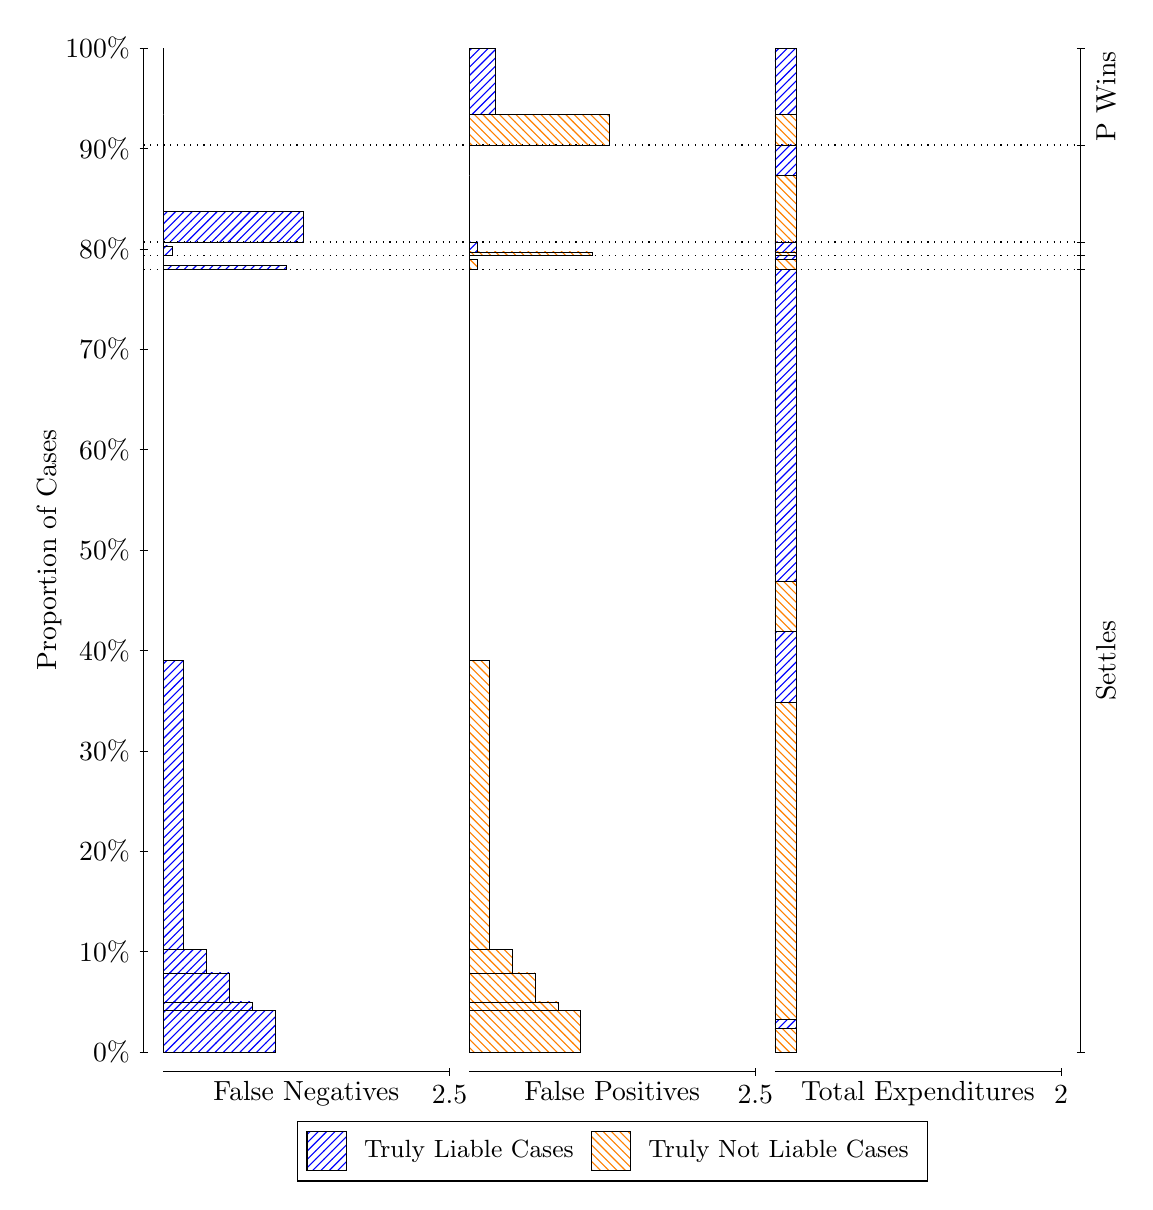
\begin{tikzpicture}
\draw[black, very thin] (1.5,1.75) -- (1.5,14.5);
\node[rotate=90, text=black, anchor=center] at (0.3, 8.125) {Proportion of Cases};
\draw[black, very thin] (1.45,1.75) -- (1.55,1.75);
\node[text=black, anchor=east] at (1.45, 1.75) {0\%};
\draw[black, very thin] (1.45,3.025) -- (1.55,3.025);
\node[text=black, anchor=east] at (1.45, 3.025) {10\%};
\draw[black, very thin] (1.45,4.3) -- (1.55,4.3);
\node[text=black, anchor=east] at (1.45, 4.3) {20\%};
\draw[black, very thin] (1.45,5.575) -- (1.55,5.575);
\node[text=black, anchor=east] at (1.45, 5.575) {30\%};
\draw[black, very thin] (1.45,6.85) -- (1.55,6.85);
\node[text=black, anchor=east] at (1.45, 6.85) {40\%};
\draw[black, very thin] (1.45,8.125) -- (1.55,8.125);
\node[text=black, anchor=east] at (1.45, 8.125) {50\%};
\draw[black, very thin] (1.45,9.4) -- (1.55,9.4);
\node[text=black, anchor=east] at (1.45, 9.4) {60\%};
\draw[black, very thin] (1.45,10.675) -- (1.55,10.675);
\node[text=black, anchor=east] at (1.45, 10.675) {70\%};
\draw[black, very thin] (1.45,11.95) -- (1.55,11.95);
\node[text=black, anchor=east] at (1.45, 11.95) {80\%};
\draw[black, very thin] (1.45,13.225) -- (1.55,13.225);
\node[text=black, anchor=east] at (1.45, 13.225) {90\%};
\draw[black, very thin] (1.45,14.5) -- (1.55,14.5);
\node[text=black, anchor=east] at (1.45, 14.5) {100\%};

\draw[black, very thin] (13.4,1.75) -- (13.4,14.5);
\draw[black, very thin] (13.35,1.75) -- (13.45,1.75);
\node[anchor=west] at (13.35, 1.75) {};
\draw[black, very thin] (13.35,11.689) -- (13.45,11.689);
\node[anchor=west] at (13.35, 11.689) {};
\draw[black, very thin] (13.35,11.863) -- (13.45,11.863);
\node[anchor=west] at (13.35, 11.863) {};
\draw[black, very thin] (13.35,12.037) -- (13.45,12.037);
\node[anchor=west] at (13.35, 12.037) {};
\draw[black, very thin] (13.35,13.269) -- (13.45,13.269);
\node[anchor=west] at (13.35, 13.269) {};
\draw[black, very thin] (13.35,14.5) -- (13.45,14.5);
\node[anchor=west] at (13.35, 14.5) {};

\draw[black, very thin, pattern color=blue, pattern=north east lines] (1.75,1.75) rectangle (3.167,2.2789);
\draw[black, very thin, pattern color=blue, pattern=north east lines] (1.75,2.2789) rectangle (2.8763,2.3852);
\draw[black, very thin, pattern color=blue, pattern=north east lines] (1.75,2.3852) rectangle (2.5857,2.7531);
\draw[black, very thin, pattern color=blue, pattern=north east lines] (1.75,2.7531) rectangle (2.295,3.0565);
\draw[black, very thin, pattern color=blue, pattern=north east lines] (1.75,3.0565) rectangle (2.0043,6.7196);
\draw[black, very thin, pattern color=orange, pattern=north west lines] (1.75,6.7196) rectangle (1.75,11.689);
\draw[black, very thin, pattern color=blue, pattern=north east lines] (1.75,11.689) rectangle (3.3123,11.738);
\draw[black, very thin, pattern color=orange, pattern=north west lines] (1.75,11.738) rectangle (1.75,11.863);
\draw[black, very thin, pattern color=blue, pattern=north east lines] (1.75,11.863) rectangle (1.859,11.988);
\draw[black, very thin, pattern color=orange, pattern=north west lines] (1.75,11.988) rectangle (1.75,12.037);
\draw[black, very thin, pattern color=blue, pattern=north east lines] (1.75,12.037) rectangle (3.5303,12.424);
\draw[black, very thin, pattern color=orange, pattern=north west lines] (1.75,12.424) rectangle (1.75,13.269);
\draw[black, very thin, pattern color=orange, pattern=north west lines] (1.75,13.269) rectangle (1.75,13.656);
\draw[black, very thin, pattern color=blue, pattern=north east lines] (1.75,13.656) rectangle (1.75,14.5);
\draw[black, very thin, pattern color=orange, pattern=north west lines] (5.6333,1.75) rectangle (7.0503,2.2788);
\draw[black, very thin, pattern color=orange, pattern=north west lines] (5.6333,2.2788) rectangle (6.7597,2.3852);
\draw[black, very thin, pattern color=orange, pattern=north west lines] (5.6333,2.3852) rectangle (6.469,2.7531);
\draw[black, very thin, pattern color=orange, pattern=north west lines] (5.6333,2.7531) rectangle (6.1783,3.0564);
\draw[black, very thin, pattern color=orange, pattern=north west lines] (5.6333,3.0564) rectangle (5.8877,6.7198);
\draw[black, very thin, pattern color=blue, pattern=north east lines] (5.6333,6.7198) rectangle (5.6333,11.689);
\draw[black, very thin, pattern color=orange, pattern=north west lines] (5.6333,11.689) rectangle (5.7423,11.814);
\draw[black, very thin, pattern color=blue, pattern=north east lines] (5.6333,11.814) rectangle (5.6333,11.863);
\draw[black, very thin, pattern color=orange, pattern=north west lines] (5.6333,11.863) rectangle (7.1957,11.912);
\draw[black, very thin, pattern color=blue, pattern=north east lines] (5.6333,11.912) rectangle (5.7423,12.037);
\draw[black, very thin, pattern color=orange, pattern=north west lines] (5.6333,12.037) rectangle (5.6333,12.882);
\draw[black, very thin, pattern color=blue, pattern=north east lines] (5.6333,12.882) rectangle (5.6333,13.269);
\draw[black, very thin, pattern color=orange, pattern=north west lines] (5.6333,13.269) rectangle (7.4137,13.656);
\draw[black, very thin, pattern color=blue, pattern=north east lines] (5.6333,13.656) rectangle (5.9603,14.5);
\draw[black, very thin, pattern color=orange, pattern=north west lines] (9.5167,1.75) rectangle (9.7892,2.0533);
\draw[black, very thin, pattern color=blue, pattern=north east lines] (9.5167,2.0533) rectangle (9.7892,2.1597);
\draw[black, very thin, pattern color=orange, pattern=north west lines] (9.5167,2.1597) rectangle (9.7892,6.1909);
\draw[black, very thin, pattern color=blue, pattern=north east lines] (9.5167,6.1909) rectangle (9.7892,7.0877);
\draw[black, very thin, pattern color=orange, pattern=north west lines] (9.5167,7.0877) rectangle (9.7892,7.7229);
\draw[black, very thin, pattern color=blue, pattern=north east lines] (9.5167,7.7229) rectangle (9.7892,11.689);
\draw[black, very thin, pattern color=orange, pattern=north west lines] (9.5167,11.689) rectangle (9.7892,11.814);
\draw[black, very thin, pattern color=blue, pattern=north east lines] (9.5167,11.814) rectangle (9.7892,11.863);
\draw[black, very thin, pattern color=orange, pattern=north west lines] (9.5167,11.863) rectangle (9.7892,11.912);
\draw[black, very thin, pattern color=blue, pattern=north east lines] (9.5167,11.912) rectangle (9.7892,12.037);
\draw[black, very thin, pattern color=orange, pattern=north west lines] (9.5167,12.037) rectangle (9.7892,12.882);
\draw[black, very thin, pattern color=blue, pattern=north east lines] (9.5167,12.882) rectangle (9.7892,13.269);
\draw[black, very thin, pattern color=orange, pattern=north west lines] (9.5167,13.269) rectangle (9.7892,13.656);
\draw[black, very thin, pattern color=blue, pattern=north east lines] (9.5167,13.656) rectangle (9.7892,14.5);
\draw[black, dotted] (1.5,11.689) -- (13.4,11.689);
\draw[black, dotted] (1.5,11.863) -- (13.4,11.863);
\draw[black, dotted] (1.5,12.037) -- (13.4,12.037);
\draw[black, dotted] (1.5,13.269) -- (13.4,13.269);
\draw[black, very thin] (1.75,1.5) -- (5.3833,1.5);
\node[text=black, anchor=north] at (3.5667, 1.5) {False Negatives};
\draw[black, very thin] (5.3833,1.45) -- (5.3833,1.55);
\node[text=black, anchor=north] at (5.3833, 1.45) {2.5};

\draw[black, very thin] (5.6333,1.5) -- (9.2667,1.5);
\node[text=black, anchor=north] at (7.45, 1.5) {False Positives};
\draw[black, very thin] (9.2667,1.45) -- (9.2667,1.55);
\node[text=black, anchor=north] at (9.2667, 1.45) {2.5};

\draw[black, very thin] (9.5167,1.5) -- (13.15,1.5);
\node[text=black, anchor=north] at (11.333, 1.5) {Total Expenditures};
\draw[black, very thin] (13.15,1.45) -- (13.15,1.55);
\node[text=black, anchor=north] at (13.15, 1.45) {2};

\node[text=black, centered, rotate=90] at (13.72, 6.7197) {Settles};



\node[text=black, centered, rotate=90] at (13.72, 13.884) {P Wins};

\draw (7.449999999999999,1.5) node[draw=none] (baseCoordinate) {};
\begin{scope}[align=center]
        \matrix[scale=0.5, draw=black, below=0.5cm of baseCoordinate, nodes={draw}, column sep=0.1cm]{
            \node[rectangle, draw, minimum width=0.5cm, minimum height=0.5cm, pattern color=blue, pattern=north east lines] {}; &
            \node[draw=none, font=\small, text=black] (B) {Truly Liable Cases}; &
            \node[rectangle, draw, minimum width=0.5cm, minimum height=0.5cm, pattern color=orange, pattern=north west lines] {}; &
            \node[draw=none, font=\small, text=black] (B) {Truly Not Liable Cases}; \\
            };
\end{scope}

\end{tikzpicture}
\end{document}